\documentclass[11pt]{amsart}
\pdfsuppressptexinfo=-1
\usepackage[margin=1.1in]{geometry}
\usepackage{amsmath,amssymb,amsthm,mathtools}
\usepackage{booktabs,enumitem,array}
\usepackage{tikz}
\usepackage[hidelinks]{hyperref}

\newtheorem{theorem}{Theorem}[section]
\newtheorem{lemma}[theorem]{Lemma}
\newtheorem{proposition}[theorem]{Proposition}
\newtheorem{corollary}[theorem]{Corollary}
\theoremstyle{definition}
\newtheorem{definition}[theorem]{Definition}
\theoremstyle{remark}
\newtheorem{remark}[theorem]{Remark}
\numberwithin{equation}{section}
\setlength{\emergencystretch}{2em}
\raggedbottom

\newcommand{\R}{\mathbb{R}}
\newcommand{\area}{\operatorname{area}}
\newcommand{\conv}{\operatorname{conv}}
\newcommand{\lmin}{\lambda_{\min}}
\newcommand{\Mp}{M^{+}}
\newcommand{\Mpm}{M^{\pm}}
% ---------------------------------------------------------------------------------------------------------------
\newcommand{\NCELLS}{1{,}048{,}576}
\newcommand{\NPARTS}{16{,}384}
\newcommand{\FAMMIN}{0.2420538}            % best local minimum of A found (300 starts)
\newcommand{\KELLERFAM}{0.23943903}        % Keller's numerical minimum for his four arcs
\newcommand{\GRID}{(4,2,2,16,2,2,8,2,2,8,2,2)}
\newcommand{\TAU}{0.2414}
\newcommand{\NLEAVES}{433{,}912{,}890}
\newcommand{\NNODES}{866{,}777{,}204}
\newcommand{\NKLEAVES}{70{,}576{,}243}
\newcommand{\XMAX}{0.61497885}        % root box bound (rounded outwards from 2 tau / w_T - 1/2)
\newcommand{\YMAX}{0.48280001}
\newcommand{\GAPFAM}{6.54\times10^{-4}}    % FAMMIN - TAU (rounded)
\newcommand{\MINMARGINFULL}{9.6074815\times10^{-8}}
\newcommand{\MINMARGIN}{9.60\times10^{-8}}      % smallest accepted margin, rounded down (used in inequalities)
\newcommand{\MINMARGINVAL}{9.607\times10^{-8}}  % the same, rounded down (used where the value is stated)
\newcommand{\DEPTHROWS}{}
\newcommand{\FIRSTRUNTABLE}{}
\newcommand{\RUNFACTS}{}
\newcommand{\SEARCHTIME}{about $4.0$\,h on up to $6{,}432$ CPUs, then about $1.8$\,h on $1{,}536$ CPUs}
\newcommand{\CHECKTIME}{about $12$\,min}
\newcommand{\RERUNCPU}{208}
\newcommand{\LEANCPU}{680}
\newcommand{\KCPU}{29{,}000}
\newcommand{\HWX}{0.3075}
\newcommand{\HWY}{0.2415}
\newcommand{\MBOUND}{18.9}
\newcommand{\LEANTAU}{\TAU}
\newcommand{\LEANCERT}{of Section~\ref{sec:cert}}
\newcommand{\LEANWEAKER}{, the bound of Theorem~\ref{thm:main}}
\newcommand{\LEANLEAVES}{433{,}912{,}901}
\newcommand{\leanStd}{\texttt{propext}, \texttt{Classical.choice} and \texttt{Quot.sound}}
% Proof of the bound by the kernel alone.
\newcommand{\KLEAVES}{196{,}725{,}046}      % leaves of the merged certificate
% Release slots.
\newcommand{\ZENODODOI}{10.5281/zenodo.23717801}   % Zenodo supplement record
\newcommand{\REPOURL}{https://github.com/tejasvi/moser-worm-rotations-bound/tree/v8}   % code repository, release tag
\newcommand{\COMMITREF}{}   % set by commit.tex (outside the repository) once the release commit exists: , commit + its first 12 hex digits
\IfFileExists{commit.tex}{\input{commit.tex}}{}
% ---------------------------------------------------------------------------------------------------------------
\hypersetup{pdftitle={A lower bound for Moser's worm problem with rotations and translations},
  pdfauthor={Tejasvi Singh Tomar}}

\begin{document}

\title[Moser's worm problem with rotations and translations]{A lower bound for Moser's worm problem with rotations and translations}
\author{Tejasvi Singh Tomar}
\renewcommand{\urladdrname}{{\itshape ORCID}}
\urladdr{\href{https://orcid.org/0000-0003-4668-3639}{https://orcid.org/0000-0003-4668-3639}}
\subjclass[2020]{52A10, 52A38; 65G40, 68V05, 68V20}
\keywords{Moser's worm problem, universal cover, convex hull, branch and bound, interval arithmetic, computer-assisted proof, formal verification, Lean 4}

\begin{abstract}
In its convex form, Moser's worm problem asks for the least area of a convex set in the plane that contains a copy of every arc of length~$1$. For the version in which the copies may be rotated and translated but not reflected, we prove that this least area $\Mp$ satisfies $\Mp\ge\TAU$; the best bound before, $0.239$, follows from Keller's bound for the version with reflections. The proof bounds the area of the convex hull of copies of five polygonal arcs, among them two zigzags that turn in opposite directions, so that without reflections the hull must contain a zigzag turning each way. A branch and bound over the placements of the arcs, with second-order Taylor bounds for signed areas of polygons, produces a certificate, which is checked in ball arithmetic and in the Lean proof assistant.
\end{abstract}

\maketitle

\section{Introduction}\label{sec:intro}

In 1966 Leo Moser asked for the smallest region of the plane that contains a copy of every arc of length~$1$ \cite{Mos66}, where an arc of length $\ell$ is the image of a continuous map $\gamma\colon[0,1]\to\R^2$ of length $\ell$. This is Moser's worm problem \cite{BMP05}. We consider convex regions. The answer may depend on which copies are admitted. Following Mazur \cite{Maz26}, let $\Mpm$ be the infimum of the areas of convex sets that contain a congruent copy of every arc of length~$1$, and let $\Mp$ be the infimum over convex sets that contain, for every such arc, a copy obtained by a rotation and a translation. A convex region of least area exists in both versions, by the Blaschke selection theorem \cite{NPL92,Maz26}. Since a copy obtained by a rotation and a translation is congruent, $\Mpm\le\Mp$; the two could differ, because a congruent copy may be a mirror image of the arc; whether they do is not known. The constant $\Mp$ is constant 13a of the list of optimization constants \cite{Tao26}.

Lower bounds come from finite families of arcs. A convex set that contains copies of arcs $\gamma_1,\dots,\gamma_m$ contains the convex hull of these copies, so its area is at least the least area of such a hull. Wetzel \cite{Wet73} combined the unit segment with the width of Schaer's broadworm \cite{Sch68} and obtained $0.21946$. Khandhawit and Sriswasdi \cite{KS07} obtained $0.227498$ from three arcs, and Khandhawit, Pagonakis and Sriswasdi \cite{KPS13} obtained $0.232239$. These three bounds hold in both versions, whichever motions their authors allow, because they use only arcs that are symmetric about a line and the minimal width of Schaer's broadworm. Two recent preprints, both with formalizations in Lean, go further: Mazur \cite{Maz26} reports $0.23743658$ for both $\Mpm$ and $\Mp$, and Keller \cite{Kel26} proved $\Mpm\ge0.239$ with four polygonal arcs, namely a segment~$L$, an arc~$T$ formed by two sides of an equilateral triangle, a three-link arc and a zigzag. Since $\Mpm\le\Mp$, his bound also gives $\Mp\ge0.239$. He found numerically a placement of his four arcs with hull area about $\KELLERFAM$, so no bound from these arcs can exceed about this number, also without reflections: his zigzag is the only one of his arcs that is not symmetric about a line, so a placement that reflects it can be reflected as a whole.

Upper bounds come from explicit covers. Panraksa and Wichiramala \cite{PW21} proved Wetzel's conjecture that the circular sector of radius~$1$ and angle $\pi/6$ contains a congruent copy of every unit arc, so $\Mpm\le\pi/12<0.2618$. Deng \cite{Den26} reports, in a preprint, an isosceles triangle of area $0.257883595\ldots$ with the same property. Both covers are symmetric about a line. A convex set $\Omega$ that is symmetric about a line and contains a congruent copy of an arc also contains a copy obtained by a rotation and a translation: if the copy is reflected, its mirror image in the axis of $\Omega$ is such a copy. These bounds therefore hold for $\Mp$ as well. Keller \cite{Kel26} constructed a quadrilateral of area $0.24633\ldots$ that contains a congruent copy of every unit arc, which shows $\Mpm\le0.24633\ldots$. The quadrilateral, however, is not symmetric, and his proof uses reflections \cite[Section~4]{Kel26}, so it does not give $\Mp\le0.24633\ldots$. Since $\TAU<0.24633\ldots$, the bound $\Mp\ge\TAU$ proved below does not decide whether $\Mpm<\Mp$.

Our arcs (Definition~\ref{def:arcs}), each of length $1$, are Keller's $L$ and $T$; a three-link arc $U$ that, like Keller's, has three links of length $1/3$ and changes direction twice in the same sense, by $84^\circ$ each time instead of his $82.5^\circ$; and, in place of his zigzag, two three-link zigzags $C$ and $S$. Each zigzag has two equal and parallel outer links; the link lengths of $C$ differ from those of $S$, and the two turn in opposite directions, $C$ first to the right and $S$ first to the left. When reflections are allowed, either zigzag can be reflected so that both turn the same way; when they are not, the hull must contain a zigzag turning each way. A numerical search found a placement of the five arcs, by rotations and translations, whose hull area exceeds $\TAU$ by only about $\GAPFAM$ (Section~\ref{sec:limits}), so no bound from these arcs can be much larger.

\begin{theorem}\label{thm:main}
Let $\Omega\subset\R^2$ be convex, and suppose that $\Omega$ contains, for each of the arcs $L,T,U,C,S$ of Definition~\textup{\ref{def:arcs}}, a copy obtained by a rotation and a translation. Then $\area\Omega\ge\TAU$. Consequently $\Mp\ge\TAU$.
\end{theorem}

\subsection*{The method}
We fix the segment $L$ and normalize the placements of the other four arcs, so that a placement is a point $p\in\R^{12}$, given by an angle and a translation for each of $T$, $U$, $C$ and $S$. Let $A(p)$ be the area of the convex hull of the placed arcs. An adaptation of a chord estimate of Keller confines the placements with $A(p)<\TAU$ to a box $X$, and we prove $A>\TAU$ on $X$ by a branch and bound over subboxes. On a box we bound $A$ from below by the signed area of a polygon spanned by vertices of the placed arcs, under conditions that make it at most $A$ on the whole box. We bound this signed area from below by its first-order Taylor polynomial at the centre of the box minus a bound for the remainder, which we obtain from the Hessian at the centre and a bound for the variation of the Hessian over the box. Where the hull changes its combinatorial type inside a box, we take a convex combination of such bounds for several polygons before bounding its linear part over the box, so that the gradients can partly cancel. Keller \cite{Kel26} bounds the polygon areas on a box by polynomials of degree at most two in the translations and in the cosines and sines of the angle offsets, and he also combines the bounds of several polygons with weights; in place of his polynomial bounds we use Taylor bounds, as in our proof of a lower bound for Lebesgue's universal covering problem \cite{Tom26}.

\subsection*{Verification}
A checker in ball arithmetic, which shares no code with the search program, verifies the certificate \cite{TomData} (Section~\ref{sec:cert}), and the bound $\Mp\ge\TAU$ is proved twice in the Lean~4 proof assistant, including the reduction of Section~\ref{sec:reduction} and the polygon bounds of Section~\ref{sec:box}: once with a checker written in Lean whose runs are executed as compiled code, and once with every check run by Lean's kernel (Section~\ref{sec:lean}).

Section~\ref{sec:reduction} reduces Theorem~\ref{thm:main} to a statement about a box of placements. Section~\ref{sec:box} proves the polygon bounds and their versions on a box. Section~\ref{sec:cert} describes the certificate and the checker and proves Theorem~\ref{thm:main}. Section~\ref{sec:lean} describes the formal proofs. Section~\ref{sec:limits} records numerical observations that the proof does not use. The appendix gives the format of the certificate, bounds the effect of the two steps of the checker that leave ball arithmetic (a fallback for square roots and one rounding to double precision), and describes the leaf test of the formal proof.

\section{Reduction to a box of placements}\label{sec:reduction}

For $a,b\in\R^2$ put $\det(a,b)=a_1b_2-a_2b_1$. Let $u(\varphi)=(\cos\varphi,\sin\varphi)$, let $R_\varphi$ be the rotation of $\R^2$ about the origin by the angle $\varphi$, and let $J=R_{\pi/2}$. Rotations preserve $\det$, and $J$ commutes with every $R_\varphi$. We write $\area$ for the Lebesgue measure on $\R^2$, $\conv$ for the convex hull and $|\cdot|$ for the Euclidean norm. A \emph{proper motion} is a map $x\mapsto R_\varphi x+t$. For points $v_0,\dots,v_n$ we write $[v_0,\dots,v_n]$ for the polygonal arc that runs through them in this order. For a point $v$, lengths $\ell_1,\dots,\ell_n>0$ and angles $\alpha_1,\dots,\alpha_n$ in degrees, the polygonal arc \emph{starting at $v$ with these lengths and directions} is $[v_0,\dots,v_n]$ with $v_0=v$ and $v_k=v_{k-1}+\ell_k\,u(\pi\alpha_k/180)$.

\begin{definition}\label{def:arcs}
The arcs $L,T,U,C,S$ are the polygonal arcs starting at the given point with the given lengths and directions:
\begin{center}
\begin{tabular}{@{}llll@{}}
\toprule
Arc & Start & Lengths & Directions (degrees)\\
\midrule
$L$ & $(-1/2,0)$ & $1$ & $0$\\
$T$ & $(-1/4,0)$ & $1/2,\ 1/2$ & $60,\ -60$\\
$U$ & $(0,0)$ & $1/3,\ 1/3,\ 1/3$ & $0,\ 84,\ 168$\\
$C$ & $(0,0)$ & $3/20,\ 7/10,\ 3/20$ & $0,\ -70,\ 0$\\
$S$ & $(0,0)$ & $41/250,\ 84/125,\ 41/250$ & $0,\ 75,\ 0$\\
\bottomrule
\end{tabular}
\end{center}
\end{definition}

The shapes of $U$, $C$ and $S$ come from a numerical search for arcs whose smallest hull area, together with $L$ and $T$, is large, with the parameters rounded to simple values. The target $\tau=\TAU$ lies below the smallest hull area of the five arcs that we found (Section~\ref{sec:limits}); the certificate grows quickly as $\tau$ approaches that area.

\begin{figure}[ht]
\centering
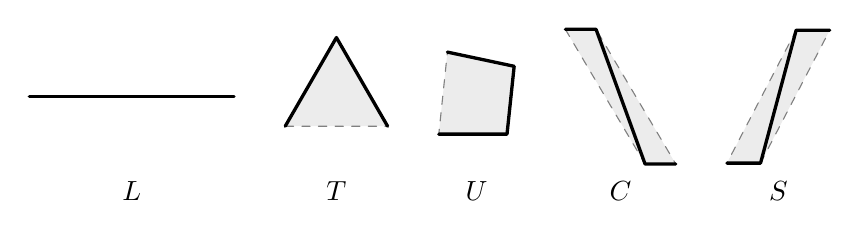
\begin{tikzpicture}[scale=2.6,line cap=round,line join=round]
\fill[gray!15] (0.0000,0.0000) -- (1.0000,0.0000) -- cycle;
\draw[dashed,gray] (0.0000,0.0000) -- (1.0000,0.0000) -- cycle;
\draw[very thick] (0.0000,0.0000) -- (1.0000,0.0000);
\node at (0.5000,-0.46) {$L$};
\fill[gray!15] (1.2500,-0.1443) -- (1.7500,-0.1443) -- (1.5000,0.2887) -- cycle;
\draw[dashed,gray] (1.2500,-0.1443) -- (1.7500,-0.1443) -- (1.5000,0.2887) -- cycle;
\draw[very thick] (1.2500,-0.1443) -- (1.5000,0.2887) -- (1.7500,-0.1443);
\node at (1.5000,-0.46) {$T$};
\fill[gray!15] (2.0000,-0.1831) -- (2.3333,-0.1831) -- (2.3682,0.1484) -- (2.0421,0.2177) -- cycle;
\draw[dashed,gray] (2.0000,-0.1831) -- (2.3333,-0.1831) -- (2.3682,0.1484) -- (2.0421,0.2177) -- cycle;
\draw[very thick] (2.0000,-0.1831) -- (2.3333,-0.1831) -- (2.3682,0.1484) -- (2.0421,0.2177);
\node at (2.1841,-0.46) {$U$};
\fill[gray!15] (2.6182,0.3289) -- (3.0076,-0.3289) -- (3.1576,-0.3289) -- (2.7682,0.3289) -- cycle;
\draw[dashed,gray] (2.6182,0.3289) -- (3.0076,-0.3289) -- (3.1576,-0.3289) -- (2.7682,0.3289) -- cycle;
\draw[very thick] (2.6182,0.3289) -- (2.7682,0.3289) -- (3.0076,-0.3289) -- (3.1576,-0.3289);
\node at (2.8879,-0.46) {$C$};
\fill[gray!15] (3.4076,-0.3246) -- (3.5716,-0.3246) -- (3.9095,0.3246) -- (3.7455,0.3246) -- cycle;
\draw[dashed,gray] (3.4076,-0.3246) -- (3.5716,-0.3246) -- (3.9095,0.3246) -- (3.7455,0.3246) -- cycle;
\draw[very thick] (3.4076,-0.3246) -- (3.5716,-0.3246) -- (3.7455,0.3246) -- (3.9095,0.3246);
\node at (3.6586,-0.46) {$S$};
\end{tikzpicture}

\medskip
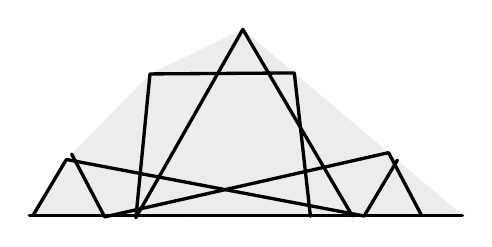
\begin{tikzpicture}[scale=5.5,line cap=round,line join=round]
\fill[gray!15] (-0.5000,0.0000) -- (-0.3260,-0.0039) -- (-0.2539,-0.0056) -- (-0.2539,-0.0056) -- (0.1491,-0.0027) -- (0.2461,-0.0020) -- (0.2732,-0.0018) -- (0.5000,0.0000) -- (0.3295,0.1444) -- (0.1119,0.3285) -- (-0.0070,0.4292) -- (-0.2214,0.3262) -- (-0.4145,0.1287) -- cycle;
\draw[very thick] (-0.5000,0.0000) -- (0.5000,0.0000); % L
\draw[very thick] (-0.2539,-0.0056) -- (-0.0070,0.4292) -- (0.2461,-0.0020); % T
\draw[very thick] (0.1491,-0.0027) -- (0.1119,0.3285) -- (-0.2214,0.3262) -- (-0.2539,-0.0056); % U
\draw[very thick] (-0.4912,-0.0002) -- (-0.4145,0.1287) -- (0.2732,-0.0018) -- (0.3499,0.1271); % C
\draw[very thick] (0.4058,-0.0008) -- (0.3295,0.1444) -- (-0.3260,-0.0039) -- (-0.4023,0.1412); % S
\end{tikzpicture}
\caption{Top: the arcs $L,T,U,C,S$ of Definition~\ref{def:arcs}, at the same scale, with their convex hulls shaded. Bottom: the placement of smallest hull area found (Section~\ref{sec:limits}); the shaded region is the convex hull of the five placed arcs.}\label{fig:arcs}
\end{figure}

Each arc has length $1$ (Figure~\ref{fig:arcs}). The convex hull of $L$ is a segment, that of $T$ is an equilateral triangle of side $1/2$, that of $U$ is an isosceles trapezoid, and those of $C$ and $S$ are parallelograms, because the first and the last link of these arcs are parallel and have equal length. Every vertex of $T$, $U$, $C$ and $S$ is a vertex of its convex hull.

We number the arcs as bodies $0,\dots,4$ in the order $L,T,U,C,S$. Let $v_{i,0},\dots,v_{i,n_i}$ be the vertices of body $i$, and for $i\ge1$ let $c_i$ be the mean of all these vertices and $q_{i,j}=v_{i,j}-c_i$. For $i=0$ put $q_{0,j}=v_{0,j}$. A \emph{placement} is a vector
\[
p=(\varphi_1,t_1,\varphi_2,t_2,\varphi_3,t_3,\varphi_4,t_4)\in\R^{12},
\]
with $\varphi_i\in\R$ and $t_i\in\R^2$. We put $\varphi_0=0$ and $t_0=0$. In the placement $p$, vertex $j$ of body $i$ is at
\[
x_{i,j}(p)=R_{\varphi_i}q_{i,j}+t_i,
\]
and body $i$ occupies the arc $\gamma_i(p)$ through these points, which is the image of the arc of Definition~\ref{def:arcs} under a proper motion. Let
\[
K(p)=\conv\bigl\{x_{i,j}(p): 0\le i\le4,\ 0\le j\le n_i\bigr\}\qquad\text{and}\qquad A(p)=\area K(p).
\]
The convex hull of a polygonal arc is the convex hull of its vertices, so $K(p)$ is the convex hull of the five placed arcs.

\begin{lemma}\label{lem:family}
Let $\Omega$ be as in Theorem~\textup{\ref{thm:main}}. Then $\area\Omega\ge\inf_pA(p)$.
\end{lemma}

\begin{proof}
Let $g_0,\dots,g_4$ be proper motions with $g_i(\gamma_i)\subseteq\Omega$, where $\gamma_i$ is body $i$ in the position of Definition~\ref{def:arcs}. The set $g_0^{-1}(\Omega)$ is convex, has the same area as $\Omega$, and contains $L$ and the arcs $g_0^{-1}g_i(\gamma_i)$. The proper motion $g_0^{-1}g_i$ maps $\gamma_i$ to $R_\varphi(\gamma_i-c_i)+t$ for some $\varphi$ and $t$. So $g_0^{-1}(\Omega)$ contains the five arcs of some placement $p$, hence $K(p)$, and $\area\Omega\ge A(p)$.
\end{proof}

The \emph{extent} of a compact set $E\ne\emptyset$ in the direction of a unit vector $u$ is $\max_{x\in E}u\cdot x-\min_{x\in E}u\cdot x$.

\begin{lemma}[Chord bound {\cite[Lemma~3.2]{Kel26}}]\label{lem:chordbound}
Let $K\subseteq\R^2$ be convex and contain a segment of length $d>0$ and a compact set $E\ne\emptyset$. If $E$ has extent $\omega$ in the direction perpendicular to the segment, then $\area K\ge d\omega/2$.
\end{lemma}

\begin{proof}
Let $E'$ be the union of $E$ and the endpoints of the segment, and let $\ell_+,\ell_-\ge0$ be the largest distances from the line of the segment of the points of $E'$ in the two closed half-planes bounded by this line. Then $\ell_++\ell_-\ge\omega$. The segment and two points at these distances span triangles $\Delta_\pm\subseteq K$, possibly degenerate, with disjoint interiors and areas $d\ell_\pm/2$.
\end{proof}

For $\tau>0$ let $w_T=\sqrt3/4$, $X_\tau=2\tau/w_T-1/2$ and $Y_\tau=2\tau$, and let $D_\tau\subset\R^{12}$ be the set of placements with
\begin{gather*}
\varphi_1\in[0,\pi/3],\qquad\varphi_2\in[0,2\pi],\qquad\varphi_3,\varphi_4\in[0,\pi],\\
t_i\in[-X_\tau,X_\tau]\times[-Y_\tau,Y_\tau]\quad(1\le i\le4).
\end{gather*}

\begin{proposition}\label{prop:domain}
Let $\tau>0$. If $A(p)<\tau$ for some placement $p$, then $A(p')=A(p)$ for some $p'\in D_\tau$.
\end{proposition}

\begin{proof}
We follow Keller's argument \cite[Section~3.2]{Kel26}, omitting the reflections. The equilateral triangle $\conv T$ is invariant under the rotation by $2\pi/3$ about its centre $c_1$, and the parallelograms $\conv C$ and $\conv S$ are invariant under the half-turns about their centres $c_3$ and $c_4$. The centre of a parallelogram is the mean of its vertices, and so is the centre of an equilateral triangle. Hence $K(p)$ does not change if $\varphi_1$ is changed by a multiple of $2\pi/3$, $\varphi_3$ or $\varphi_4$ by a multiple of $\pi$, or $\varphi_2$ by a multiple of $2\pi$. The half-turn $x\mapsto-x$ is a proper motion that maps $L$ onto itself, and it maps the placed arcs of $p$ to those of the placement with angles $\varphi_i+\pi$ and translations $-t_i$, with the same hull area. Since $\pi\equiv\pi/3\pmod{2\pi/3}$, after this half-turn if necessary and the reductions above we may assume $\varphi_1\in[0,\pi/3]$, $\varphi_2\in[0,2\pi]$ and $\varphi_3,\varphi_4\in[0,\pi]$.

Let $p'$ be the placement obtained in this way, so that $A(p')=A(p)<\tau$, let $t_1,\dots,t_4$ be its translations and let $K'=K(p')$. The triangle $\conv T$ has extent at least $w_T=\sqrt3/4$ in every direction, and so does its placed copy in $K'$. Lemma~\ref{lem:chordbound}, applied to a chord of $K'$ of length $\operatorname{diam}K'$ and to this copy, gives $\operatorname{diam}K'\le2\area K'/w_T<2\tau/w_T$. For $i\ge1$ the vectors $q_{i,j}$ have mean $0$, so $t_i$ is the mean of the placed vertices of body $i$, and $t_i\in K'$. With $a_\pm=(\pm1/2,0)$, the endpoints of $L$, we get $|t_{i,1}|+1/2\le\max_\pm|t_i-a_\pm|\le\operatorname{diam}K'<2\tau/w_T$, and therefore $|t_{i,1}|<X_\tau$. The triangle $\conv\{a_-,a_+,t_i\}\subseteq K'$ has area $|t_{i,2}|/2$, so $|t_{i,2}|<2\tau=Y_\tau$. Hence $p'\in D_\tau$.
\end{proof}

\begin{corollary}\label{cor:root}
Let $\tau>0$ and let $X$ be a box with $D_\tau\subseteq X$. If $A>\tau$ on $X$, then every $\Omega$ as in Theorem~\textup{\ref{thm:main}} has $\area\Omega\ge\tau$.
\end{corollary}

\begin{proof}
If $A(p)<\tau$ for some $p$, then $A(p')<\tau$ for some $p'\in D_\tau\subseteq X$ by Proposition~\ref{prop:domain}, a contradiction. Therefore $A\ge\tau$ everywhere, and Lemma~\ref{lem:family} gives $\area\Omega\ge\tau$.
\end{proof}

\section{The box bound}\label{sec:box}

In this section we bound $A$ from below on a box of placements. A \emph{box} is a set $B=\prod_{a=1}^{12}[c_a-h_a,c_a+h_a]$ with centre $c$ and half-widths $h_a\ge0$. A \emph{vertex list} is a sequence $P=(g_1,\dots,g_m)$ of distinct vertices $g_j=(i_j,k_j)$ of the five bodies. At a placement $p$ its points are $x_j(p)=x_{i_j,k_j}(p)$, indices are taken modulo $m$, and its \emph{signed area} is
\[
F_P(p)=\frac12\sum_{j=1}^m\det\bigl(x_j(p),x_{j+1}(p)\bigr).
\]
All points $x_j(p)$ lie in $K(p)$. The following four lemmas give conditions for $F_P\le A$. The \emph{angle} from a nonzero vector $v$ to a nonzero vector $v'$ with $\det(v,v')>0$ is the number $\theta\in(0,\pi)$ with $v'/|v'|=R_\theta(v/|v|)$.

\begin{lemma}[Small lists {\cite[Lemma~3.3]{Kel26}}]\label{lem:small}
Let $x_1,\dots,x_m$ be points of a convex set $K$ with $m\le4$. Then $\frac12\sum_{j=1}^m\det(x_j,x_{j+1})\le\area K$.
\end{lemma}

\begin{proof}
For $m\le2$ the sum is $0$. For $m=3$ its absolute value is the area of the triangle $\conv\{x_1,x_2,x_3\}\subseteq K$. For $m=4$ the sum equals $\frac12\det(x_3-x_1,x_4-x_2)$. If $x_1=x_3$ this is $0$. Otherwise its absolute value is $d\omega/2$, where $d=|x_3-x_1|$ and $\omega$ is the extent of $\{x_2,x_4\}$ perpendicular to $[x_1,x_3]$, and Lemma~\ref{lem:chordbound} applies.
\end{proof}

\begin{lemma}[Fan lemma; cf.\ {\cite[Lemma~3.1]{Tom26}}]\label{lem:fan}
Let $K\subset\R^2$ be convex, let $x_1,\dots,x_m\in K$ with $m\ge3$, and let $z\in\R^2$. Suppose that $\det(x_j-z,x_{j+1}-z)>0$ for all $j$, and let $\theta_j$ be the angle from $x_j-z$ to $x_{j+1}-z$. If $\theta_1+\dots+\theta_m=2\pi$, then
\[
\area K\ \ge\ \frac12\sum_{j=1}^m\det(x_j-z,x_{j+1}-z)\ =\ \frac12\sum_{j=1}^m\det(x_j,x_{j+1}).
\]
\end{lemma}

\begin{proof}
Write $x_1-z=r_1u(\psi_1)$ with $r_1>0$, and put $\psi_{j+1}=\psi_j+\theta_j$. Then $x_j-z=r_ju(\psi_j)$ with $r_j>0$, and $\psi_{m+1}=\psi_1+2\pi$. The intervals $(\psi_j,\psi_{j+1})$ are disjoint subintervals of $[\psi_1,\psi_1+2\pi)$ of length less than $\pi$. Every direction from $z$ lies in one of the closed sectors $\{z+s\,u(\psi):s\ge0,\ \psi_j\le\psi\le\psi_{j+1}\}$, so the points $x_j-z$ do not lie in an open half-plane bounded by a line through $0$, and $z\in\conv\{x_1,\dots,x_m\}\subseteq K$. Hence the triangle $\Delta_j=\conv\{z,x_j,x_{j+1}\}$ lies in $K$. Its interior lies in the open sector between the directions $\psi_j$ and $\psi_{j+1}$, so the triangles have disjoint interiors, and $\area K\ge\sum_j\area\Delta_j=\frac12\sum_j\det(x_j-z,x_{j+1}-z)$. Finally, $\sum_j\det(x_j-z,x_{j+1}-z)=\sum_j\det(x_j,x_{j+1})+\sum_j\det(z,x_j)-\sum_j\det(z,x_{j+1})$, and the last two sums are equal.
\end{proof}

\begin{lemma}[Fan from a vertex {\cite[Lemma~3.4]{Kel26}}]\label{lem:vfan}
Let $x_1,\dots,x_m$ be points of a convex set $K$ with $m\ge3$, and put $\xi_j=x_j-x_1$. If $\det(\xi_2,\xi_j)>0$ for $3\le j\le m$ and $\det(\xi_j,\xi_{j+1})>0$ for $3\le j\le m-1$, then $\frac12\sum_{j=1}^m\det(x_j,x_{j+1})=\sum_{j=2}^{m-1}\area\conv\{x_1,x_j,x_{j+1}\}\le\area\conv\{x_1,\dots,x_m\}$.
\end{lemma}

\begin{proof}
The vectors $\xi_j$ with $j\ge3$ lie in the open half-plane to the left of $\xi_2$, and their angles from $\xi_2$ increase strictly with $j$. Consequently, the triangles $\conv\{x_1,x_j,x_{j+1}\}$ have disjoint interiors and positive areas $\frac12\det(\xi_j,\xi_{j+1})$, and the shoelace sum of the list equals the sum of these areas.
\end{proof}

\begin{lemma}[Chord decomposition {\cite[Lemma~3.5]{Kel26}}]\label{lem:chord}
Let $x_1,\dots,x_m$ be points of a convex set $K$, and let $1\le s,s'\le m$ with $2\le s'-s\pmod m\le m-2$. Let $P'$ be the list $x_s,x_{s+1},\dots,x_{s'}$ and $P''$ the list $x_{s'},x_{s'+1},\dots,x_s$, with indices modulo $m$. Suppose that $x_s\ne x_{s'}$, that the points of $P'$ strictly between $x_s$ and $x_{s'}$ satisfy $\det(x_{s'}-x_s,x-x_s)\le0$ and those of $P''$ strictly between $x_{s'}$ and $x_s$ satisfy $\det(x_{s'}-x_s,x-x_s)\ge0$, and that the signed areas of $P'$ and $P''$ are at most the areas of the convex hulls of their points. Then $\frac12\sum_{j=1}^m\det(x_j,x_{j+1})\le\area\conv\{x_1,\dots,x_m\}$.
\end{lemma}

\begin{proof}
The signed area of the list is the sum of the signed areas of $P'$ and $P''$, because the chord appears in the two shoelace sums with opposite orientations. The convex hulls of $P'$ and $P''$ lie in the two closed half-planes bounded by the line through $x_s$ and $x_{s'}$, so they meet in a set of area $0$, and both lie in $\conv\{x_1,\dots,x_m\}$.
\end{proof}

By Lemmas~\ref{lem:small} and~\ref{lem:vfan}, the hypothesis of Lemma~\ref{lem:chord} on $P'$ and $P''$ holds if each of them has at most four points, satisfies the conditions of Lemma~\ref{lem:vfan} after a cyclic shift, or can itself be cut by Lemma~\ref{lem:chord}. We call a vertex list together with such a recipe, or with a point $z$ for Lemma~\ref{lem:fan}, a \emph{structure}, and we say that a structure is \emph{valid} at $p$ if the hypotheses of the corresponding lemma hold for the points $x_j(p)$. If a structure with vertex list $P$ is valid at $p$, then $F_P(p)\le A(p)$.

On a box the validity conditions are strict inequalities between determinants of the points $x_j(p)$. We bound how much they can change. For a body $i\ge1$ let $r_i$ be the half-width of $B$ in $\varphi_i$, and let $\delta_i=(h_{i,1}^2+h_{i,2}^2)^{1/2}$, where $h_{i,1},h_{i,2}$ are the half-widths of $B$ in the coordinates of $t_i$. Put $r_0=\delta_0=0$. For a vertex $g=(i,k)$ let $\mu(g)=|q_{i,k}|\,r_i+\delta_i$. For a function $\phi$ on $B$ and $p\in B$ write $\Delta\phi=\phi(p)-\phi(c)$.

\begin{lemma}[Variation of determinants; cf.\ {\cite[Lemma~3.6]{Tom26}}]\label{lem:detvar}
Let $B$ be a box with centre $c$ and $p\in B$.
\begin{enumerate}[label=\textup{(\alph*)},leftmargin=*]
\item $\|R_{\varphi_i(p)}-R_{\varphi_i(c)}\|\le r_i$, $|\Delta t_i|\le\delta_i$ and $|\Delta x_g|\le\mu(g)$ for every vertex~$g$.
\item For vertices $g,g'$ let $\mu(g,g')=|q_{i,k'}-q_{i,k}|\,r_i$ if $g=(i,k)$ and $g'=(i,k')$ lie on the same body, and $\mu(g,g')=\mu(g)+\mu(g')$ otherwise. Then $|\Delta(x_{g'}-x_g)|\le\mu(g,g')$.
\item For vertices $a,b,g$ put $u=x_b-x_a$ and $v=x_g-x_a$. Then $|\Delta\det(u,v)|\le\mu(a,b)|v(c)|+\mu(a,g)|u(c)|+\mu(a,b)\mu(a,g)$, and $\Delta\det(u,v)=0$ if $a,b,g$ lie on one body.
\item For a point $z$ and consecutive vertices $g=(i,k)$, $g'=(i',k')$ of a list, with positions $x$ and $y$, let $\eta=\det(x-z,y-z)$. If $i=i'=0$, then $\Delta\eta=0$. If $i=i'\ge1$, then $|\Delta\eta|\le|q_{i,k'}-q_{i,k}|\bigl(\delta_i(1+r_i)+|t_i(c)-z|\,r_i\bigr)$. If $i\ne i'$, then $|\Delta\eta|\le\mu(g)\bigl(|y(c)-z|+\mu(g')\bigr)+|x(c)-z|\,\mu(g')$.
\end{enumerate}
\end{lemma}

\begin{proof}
(a) $\|R_\varphi-R_{\varphi'}\|=2|\sin((\varphi-\varphi')/2)|\le|\varphi-\varphi'|$, so $|\Delta x_g|\le\|\Delta R_{\varphi_i}\|\,|q_{i,k}|+|\Delta t_i|\le\mu(g)$. (b) On one body $x_{g'}-x_g=R_{\varphi_i}(q_{i,k'}-q_{i,k})$; otherwise use (a) twice. (c) $\Delta\det(u,v)=\det(\Delta u,v(c))+\det(u(c),\Delta v)+\det(\Delta u,\Delta v)$ and (b). If $a=(i,a')$, $b=(i,b')$ and $g=(i,g')$ lie on one body, then $\det(u,v)=\det(q_{i,b'}-q_{i,a'},q_{i,g'}-q_{i,a'})$ is constant. (d) If $i=i'\ge1$, then $\eta=\det(q_{i,k},q_{i,k'})+\det(t_i-z,R_{\varphi_i}w)$ with $w=q_{i,k'}-q_{i,k}$, because $\det(Ra+t,Rb+t)=\det(a,b)+\det(t,R(b-a))$ for a rotation $R$. Writing $R=R_{\varphi_i}$ and $R_c=R_{\varphi_i(c)}$, $\Delta\eta=\det(\Delta t_i,R_cw)+\det(t_i(c)-z,(R-R_c)w)+\det(\Delta t_i,(R-R_c)w)$, and (a) bounds the three terms. If $i\ne i'$, then $\Delta\eta=\det(\Delta x,y-z)+\det(x(c)-z,\Delta y)$ and $|y-z|\le|y(c)-z|+\mu(g')$.
\end{proof}

\begin{lemma}[Validity on a box]\label{lem:valid}
Let $B$ be a box with centre $c$, and let a structure satisfy the following. A fan has at least three points, a fan from a vertex at least three and a small list or piece at most four, and every cut satisfies the condition on $s$ and $s'$ of Lemma~\textup{\ref{lem:chord}}. At $c$, every determinant in its validity conditions that must be positive exceeds the bound of Lemma~\textup{\ref{lem:detvar}(c)} or~\textup{(d)} for its change, every determinant that must be $\le0$ or $\ge0$ satisfies the corresponding inequality with this bound added or subtracted, every pair of chord endpoints satisfies $|x_{s'}(c)-x_s(c)|>\mu(g_s,g_{s'})$, and, for a fan, the angles at $c$ add up to $2\pi$. Then the structure is valid at every $p\in B$, and $F_P\le A$ on $B$.
\end{lemma}

\begin{proof}
The conditions on the numbers of points do not depend on $p$. By Lemma~\ref{lem:detvar} every other condition holds on $B$, except possibly the angle sum of a fan. For the angle sum we use the argument of \cite[Lemma~3.3]{Tom26}. For a fan let $\Theta(p)$ be the sum of the angles at $p$. It is continuous on $B$, because the determinants are positive there, and it is an integer multiple of $2\pi$, since rotating the direction of $x_1(p)-z$ successively by the angles returns it to itself. As $B$ is connected, $\Theta=\Theta(c)=2\pi$ on $B$.
\end{proof}

We now bound $F_P$ on a box. We split the cyclic vertex list into maximal \emph{runs} of consecutive vertices on the same body. Suppose that the vertices lie on at least two bodies; then consecutive runs lie on different bodies, also cyclically. Let run $\varrho$ lie on body $\iota_\varrho$ and consist of the vertices with positions $x_{\alpha_\varrho},\dots,x_{\beta_\varrho}$, with $q$-values $q_{\alpha_\varrho},\dots,q_{\beta_\varrho}$. The identity $\det(Ra+t,Rb+t)=\det(a,b)+\det(t,R(b-a))$, summed over a run, gives
\begin{equation}\label{eq:runs}
F_P(p)=\frac12\sum_\varrho\Bigl(C_\varrho+\det\bigl(t_{\iota_\varrho},R_{\varphi_{\iota_\varrho}}w_\varrho\bigr)+\det\bigl(x_{\beta_\varrho}(p),x_{\alpha_{\varrho+1}}(p)\bigr)\Bigr),
\end{equation}
where $C_\varrho=\sum_{j=\alpha_\varrho}^{\beta_\varrho-1}\det(q_j,q_{j+1})$ and $w_\varrho=q_{\beta_\varrho}-q_{\alpha_\varrho}$. We call $\frac12\det(t_{\iota_\varrho},R_{\varphi_{\iota_\varrho}}w_\varrho)$ a \emph{run term}; it depends on the parameters of one body and vanishes for the segment. We call $\frac12\det(x_{\beta_\varrho}(p),x_{\alpha_{\varrho+1}}(p))$ a \emph{transition term}; it depends on the parameters of two different bodies. Lemma~3.4 and equation~(3.1) of \cite{Tom26} give the same identity; here all four bodies rotate.

\begin{lemma}[Taylor bound; cf.\ {\cite[Lemma~3.5]{Tom26}}]\label{lem:taylor}
Let $B$ be a box with centre $c$ and half-widths $h$, and let $F$ be twice continuously differentiable near $B$. Put $H=\nabla^2F(c)$ and $M=\operatorname{diag}(h)\,H\operatorname{diag}(h)$, let $W$ be a symmetric matrix with $|\partial_a\partial_bF(\xi)-H_{ab}|\le W_{ab}$ for all $\xi\in B$, and let $n_h$ be the number of $a$ with $h_a>0$. Let $\Lambda$ be one of the numbers
\[
\Lambda_1=\min(0,\lmin(H))\sum_ah_a^2,\quad \Lambda_2=\sum_a\min(0,M_{aa})-\sum_{a\ne b}|M_{ab}|,\quad \Lambda_3=\min(0,\lmin(M))\,n_h,
\]
or a lower bound for one of them, and put $\varepsilon=-\frac\Lambda2+\frac12\sum_{a,b}W_{ab}h_ah_b$. Then $F(p)\ge F(c)+\nabla F(c)\cdot(p-c)-\varepsilon\ge F(c)-\sum_a|\partial_aF(c)|h_a-\varepsilon$ for all $p\in B$.
\end{lemma}

\begin{proof}
Let $p\in B$ and $v=p-c=\operatorname{diag}(h)\,y$ with $|y_a|\le1$, where we take $y_a=0$ if $h_a=0$. Taylor's theorem gives $\xi\in B$ with $F(p)=F(c)+\nabla F(c)\cdot v+\frac12v^T\nabla^2F(\xi)v$. Here $v^T(\nabla^2F(\xi)-H)v\ge-\sum_{a,b}W_{ab}h_ah_b$, and $v^THv=y^TMy$ is at least each of $\Lambda_1$, $\Lambda_2$ and $\Lambda_3$: $v^THv\ge\lmin(H)|v|^2\ge\Lambda_1$; $y^TMy=\sum_aM_{aa}y_a^2+\sum_{a\ne b}M_{ab}y_ay_b\ge\Lambda_2$; and $y^TMy\ge\lmin(M)|y|^2\ge\Lambda_3$, since $|y|^2\le n_h$. Finally, $\nabla F(c)\cdot v\ge-\sum_a|\partial_aF(c)|h_a$.
\end{proof}

In \cite[Lemma~3.5]{Tom26} only $\Lambda_1$ is used.

For the bound $W$ we need the second derivatives of the terms of \eqref{eq:runs} and their variation on $B$.

\begin{lemma}[Derivatives and variation bounds]\label{lem:deriv}
Let $B$ be a box with centre $c$, and let $p\in B$.
\begin{enumerate}[label=\textup{(\alph*)},leftmargin=*]
\item Let $G=\frac12\det(t_i,R_{\varphi_i}w)$ be a run term with $i\ge1$. Its second derivatives that do not vanish identically are $\partial^2G/\partial\varphi_i^2=-\frac12\det(t_i,R_{\varphi_i}w)$ and $\partial^2G/\partial\varphi_i\,\partial t_{i,a}=\frac12\det(e_a,JR_{\varphi_i}w)$, where $e_1,e_2$ is the standard basis of $\R^2$, and on $B$
\[
\Bigl|\Delta\frac{\partial^2G}{\partial\varphi_i^2}\Bigr|\le\frac{|w|}2\bigl(\delta_i(1+r_i)+|t_i(c)|\,r_i\bigr),\qquad\Bigl|\Delta\frac{\partial^2G}{\partial\varphi_i\,\partial t_{i,a}}\Bigr|\le\frac{|w|}2\,r_i\quad(a=1,2).
\]
\item Let $G=\frac12\det(x,y)$ be a transition term, where $x$ is the position of a vertex $g=(i,k)$ and $y$ that of a vertex $g'=(i',k')$ with $i\ne i'$, and put $q=q_{i,k}$, $q'=q_{i',k'}$, $\mu=\mu(g)$ and $\mu'=\mu(g')$. The second derivatives of $G$ with respect to the coordinates of $t_i$ and $t_{i'}$ are constant. The other second derivatives $\phi$ of $G$ that do not vanish identically, and bounds for $|\Delta\phi|$ on $B$, are as follows, where $a,b\in\{1,2\}$:
\begin{align*}
\phi&=\frac{\partial^2G}{\partial\varphi_i\,\partial t_{i',b}}=\frac12\det(JR_{\varphi_i}q,e_b),&|\Delta\phi|&\le\tfrac12|q|\,r_i,\\
\phi&=\frac{\partial^2G}{\partial t_{i,a}\,\partial\varphi_{i'}}=\frac12\det(e_a,JR_{\varphi_{i'}}q'),&|\Delta\phi|&\le\tfrac12|q'|\,r_{i'},\\
\phi&=\frac{\partial^2G}{\partial\varphi_i\,\partial\varphi_{i'}}=\frac12\det(JR_{\varphi_i}q,JR_{\varphi_{i'}}q'),&|\Delta\phi|&\le\tfrac12|q|\,|q'|\,(r_i+r_{i'}),\\
\phi&=\frac{\partial^2G}{\partial\varphi_i^2}=-\frac12\det(R_{\varphi_i}q,y),&|\Delta\phi|&\le\tfrac12|q|\bigl(r_i(|y(c)|+\mu')+\mu'\bigr),\\
\phi&=\frac{\partial^2G}{\partial\varphi_{i'}^2}=-\frac12\det(x,R_{\varphi_{i'}}q'),&|\Delta\phi|&\le\tfrac12|q'|\bigl(r_{i'}(|x(c)|+\mu)+\mu\bigr).
\end{align*}
Derivatives with respect to $\varphi_i$ or $t_i$ occur only for $i\ge1$.
\end{enumerate}
\end{lemma}

\begin{proof}
Lemma~3.6(c),(d) of \cite{Tom26} gives these bounds when body~$0$ is a disk and body~$1$ does not rotate, and the same proof applies. We have $\partial_\varphi R_\varphi=R_\varphi J$ and $J^2=-I$, which gives the derivatives. Their variations are bounded with Lemma~\ref{lem:detvar}(a): for instance $|\Delta\det(R_{\varphi_i}q,y)|\le r_i|q|\,|y|+|q|\,|\Delta y|\le|q|\bigl(r_i(|y(c)|+\mu')+\mu'\bigr)$, and $\det(Ja,Jb)=\det(a,b)$ gives the third line.
\end{proof}

For a vertex list on at least two bodies, let $W$ be the symmetric matrix obtained by adding, over all run terms and transition terms of \eqref{eq:runs}, the bounds of Lemma~\ref{lem:deriv} at the corresponding entries, symmetrically. Since $\nabla^2F_P$ is the sum of the Hessians of these terms, $W$ satisfies the hypothesis of Lemma~\ref{lem:taylor}. All entries of $W$ are nonnegative.

\begin{lemma}[Eigenvalue certificate {\cite[Lemma~3.7]{Tom26}}]\label{lem:ldl}
Let $H$ be a real symmetric $d\times d$ matrix, let $\lambda\in\R$ and $N=H-\lambda I$. For $a=1,\dots,d$ define recursively
\[
L_{ab}=\frac1{D_b}\Bigl(N_{ab}-\sum_{\gamma<b}L_{a\gamma}L_{b\gamma}D_\gamma\Bigr)\quad(b<a),\qquad D_a=N_{aa}-\sum_{\gamma<a}L_{a\gamma}^2D_\gamma.
\]
If the recursion yields $D_1,\dots,D_d>0$, then $\lmin(H)>\lambda$.
\end{lemma}

\begin{proof}
The recursion gives $N=LDL^T$ with $L$ unit lower triangular and $D=\operatorname{diag}(D_1,\dots,D_d)$. For $v\ne0$ we have $L^Tv\ne0$, so $v^TNv=\sum_aD_a\bigl((L^Tv)_a\bigr)^2>0$.
\end{proof}

If the entries of $H$ are known only up to enclosing intervals and the recursion is evaluated in interval arithmetic, positive lower endpoints of the computed $D_a$ certify $\lmin(H)>\lambda$, as in \cite{Tom26}.

\begin{lemma}[Combination bound {\cite[Lemma~3.8]{Tom26}}]\label{lem:comb}
Let $B$ be a box with centre $c$ and half-widths $h$. For $s=1,\dots,n$ let a structure with vertex list $P_s$ be valid on $B$, let $F_s=F_{P_s}$, and let $\varepsilon_s\in\R$ satisfy $F_s(p)\ge F_s(c)+\nabla F_s(c)\cdot(p-c)-\varepsilon_s$ for all $p\in B$. Let $\kappa_1,\dots,\kappa_n\ge0$ with $\kappa_1+\dots+\kappa_n=1$. Then for all $p\in B$
\[
A(p)\ \ge\ \sum_{s=1}^n\kappa_s\bigl(F_s(c)-\varepsilon_s\bigr)-\sum_a\Bigl|\sum_{s=1}^n\kappa_s\partial_aF_s(c)\Bigr|h_a.
\]
\end{lemma}

\begin{proof}
$A(p)\ge F_s(p)$ for every $s$, so $A(p)\ge\sum_s\kappa_sF_s(p)\ge\sum_s\kappa_s(F_s(c)-\varepsilon_s)+u\cdot(p-c)$ with $u=\sum_s\kappa_s\nabla F_s(c)$, and $u\cdot(p-c)\ge-\sum_a|u_a|h_a$.
\end{proof}

By Lemma~\ref{lem:taylor}, the number $\varepsilon$ defined there can serve as $\varepsilon_s$. For $n=1$ the lemma gives the bound $F(c)-\sum_a|\partial_aF(c)|h_a-\varepsilon$ of Lemma~\ref{lem:taylor}.

\section{The certificate and its verification}\label{sec:cert}

\subsection{The certificate}\label{sec:certdata} The certificate for $\tau=\TAU$ is divided into parts, over which the cells of a grid on the root box $X$ are distributed (Table~\ref{tab:verif} gives the numbers). For each of its cells a part holds a binary tree of boxes, in which every inner node splits a box at the midpoint of one coordinate, and for each leaf a record with a list of structures and a list of nonnegative weights. A structure is a vertex list together with its type: a point $z$ for Lemma~\ref{lem:fan}, the marker of a small list, or a tree of cuts by Lemma~\ref{lem:chord} whose pieces are small lists or fans from a vertex (Lemma~\ref{lem:vfan}) with a given first vertex. A leaf is closed by a single structure or by several structures combined by Lemma~\ref{lem:comb}. Appendix~\ref{app:format} gives the format of a part.

\subsection{The search}\label{sec:search} The certificate was produced by a depth-first branch and bound in double precision, which is not part of the proof. At a box the search program forms candidate structures from the vertices of the convex hull at the centre and of sub-hulls of selected bodies, from small lists and from chord decompositions of the hull list, and evaluates the bound of Lemma~\ref{lem:taylor}. If no single structure closes the box, it chooses the weights of Lemma~\ref{lem:comb} for several valid structures by a linear program. A box is closed when its bound is at least $\tau+10^{-7}$, and otherwise it is split.

\subsection{The checker}\label{sec:checker} The checker works in ball arithmetic at $100$ bits of precision. The box coordinates are double-precision numbers, which are exact in Arb. Every comparison that decides whether a part is accepted is made in ball arithmetic or exactly. Two steps leave ball arithmetic, a fallback for square roots and the rounding of the number $\Lambda$ below; Appendix~\ref{app:rounding} bounds their effect. The checker reads $\tau$ as the shortest decimal number that represents the header value, here $\TAU$. For each part it performs the following steps.
\begin{enumerate}[label=(\arabic*),leftmargin=*]
\item\label{st:family} \emph{Arcs.} From the header it computes the vertices $v_{i,j}$ and the vectors $q_{i,j}$ in ball arithmetic. It verifies that each arc has length at most $1$, that body $0$ is the unit segment $L$, that body $1$ is the arc $T$, that each body whose angle range is taken modulo $\pi$ has links $(a,m,a)$ with directions $(\alpha,\beta,\alpha)$, so that its convex hull is a parallelogram whose centre is the mean of its vertices, that the numbering lists every vertex once, and that the largest length of a small list is at most $4$.
\item\label{st:root} \emph{Root box.} It verifies that $X\supseteq D_\tau$: the range of $\varphi_1$ contains $[0,\pi/3]$, for $i=2,3,4$ the range of $\varphi_i$ contains $[0,\pi p_i]$, where $p_i$ is the period of body $i$ recorded in the header, that is, $[0,2\pi]$, $[0,\pi]$ and $[0,\pi]$, and the ranges of the coordinates of every $t_i$ contain $[-X_\tau,X_\tau]$ and $[-Y_\tau,Y_\tau]$, with $X_\tau$ and $Y_\tau$ evaluated in ball arithmetic.
\item\label{st:tree} \emph{Tree.} It computes the cells of the part from the grid, the number of parts and the index of the part as in Appendix~\ref{app:format}, decodes the codes and computes the boxes, splitting each box at the double-precision midpoint of the split coordinate. It checks that every code is valid, that the array consists of complete trees with no data after the last one, that the leaf file has exactly one record for each leaf, and that the record of each leaf closed by a single structure has exactly one structure.
\item\label{st:leaf} \emph{Leaves.} At each leaf it computes the centre $c$ and the half-widths $h$ in double precision and verifies, in rational arithmetic, that $c\pm h$ are exactly the endpoints of the leaf box. It requires the record to contain at least one structure and one weight for each structure, every weight to be a nonnegative number, and at least one weight to be positive. Structures of weight $0$ are ignored. For every structure of positive weight it verifies that the vertices of its list are distinct, and it verifies the hypotheses of Lemma~\ref{lem:valid} in ball arithmetic: for a fan, the determinants $\det(x_j(c)-z,x_{j+1}(c)-z)$ exceed the bounds of Lemma~\ref{lem:detvar}(d) and the computed sum of the angles at $c$ differs from $2\pi$ by less than $1$; for a small list, it has at most four vertices; for a chord decomposition, every cut and every piece satisfies the conditions of Lemmas~\ref{lem:chord} and~\ref{lem:vfan} with the bounds of Lemma~\ref{lem:detvar}(b) and~(c). For each such structure it evaluates $F_P(c)$, $\nabla F_P(c)$ and $\nabla^2F_P(c)$ through \eqref{eq:runs}, computes $W$, and computes $\varepsilon$ by Lemma~\ref{lem:taylor} with $\Lambda$ the largest of $\Lambda_2$ and the available numbers among $\Lambda_1$ and $\Lambda_3$, where $\lmin(\nabla^2F_P(c))$ and $\lmin(M)$ are bounded from below by Lemma~\ref{lem:ldl} at a floating-point estimate lowered by $10^{-9}(1+|\lambda|)+10^{-12}$. It divides the positive weights by their sum in ball arithmetic and verifies that the right-hand side of Lemma~\ref{lem:comb} for the structures of positive weight, with these weights, exceeds $\tau$.
\end{enumerate}
If the factorization of Lemma~\ref{lem:ldl} fails for $H$ or for $M$, the corresponding number $\Lambda_1$ or $\Lambda_3$ is not used. The checker also reports, for each part, the smallest lower endpoint of the differences between the accepted bounds and $\tau$. The smallest of them, called $\delta$ in Proposition~\ref{prop:cert} below, is slightly below the threshold $10^{-7}$ of the search, because the certified bounds of the checker can be slightly smaller than the bounds that the search computes in double precision.

\subsection{Headers and coverage}\label{sec:headers}
The checks of a part were run on ranges of its leaves. Two short programs complete the verification. The presence program verifies that all parts carry the same header apart from the index of the part and that, for each part, the passing check runs on the archived files cover all of its leaves. The header program verifies that the arcs in the header are exactly those of Definition~\ref{def:arcs}, with the angle periods that step~\ref{st:root} uses, that the numbering lists every vertex once, that there is one header for each part, and that in every coordinate~$a$ the cell endpoints computed as in the checker increase with $k$ and are equal to the rational numbers $X^-_a+(X^+_a-X^-_a)k/s_a$. Adjacent cells share the endpoint computed by the same expression, so the cells tile $X$.

\subsection{Proof of Theorem~\ref{thm:main}}

\begin{proposition}\label{prop:cert}
The checker accepts every part of the certificate, the presence program and the header program accept the certificate and the check runs, and the smallest difference $\delta$ between an accepted bound and $\tau$ is $\MINMARGINFULL$.
\end{proposition}

We verified Proposition~\ref{prop:cert} by running the checker, the presence program and the header program on the archived certificate (Table~\ref{tab:verif}). All leaves were checked a second time on another machine, and a second implementation of the leaf bound, which shares no code with the checker, accepted $500$ leaves, among them those with the smallest margins.

\begin{proof}[Proof of Theorem~\ref{thm:main}]
Let $\tau=\TAU$. By the presence program all parts carry the same header, and by the header program its arcs are those of Definition~\ref{def:arcs}, its angle periods are those used in the definition of $D_\tau$, and the cells of its grid tile its root box $X$. By step~\ref{st:root}, $D_\tau\subseteq X$. By the presence program, the passing check runs of each part, for the archived files, cover all leaves of the part. By step~\ref{st:tree}, the leaves of the tree of a cell tile the cell, since each split replaces a box by its two halves. Let $B$ be a leaf; by step~\ref{st:leaf} it has centre $c$ and half-widths $h$. Consider a structure of positive weight in its record, with vertex list $P$. By step~\ref{st:leaf} and Lemma~\ref{lem:valid}, the structure is valid on $B$ and $F_P\le A$ on $B$. If the vertices of $P$ lie on at least two bodies, then \eqref{eq:runs} holds, the matrix $W$ computed by the checker bounds the variation of $\nabla^2F_P$ on $B$ by Lemma~\ref{lem:deriv}, the number $\Lambda-2^{-52}\cdot19$ is a lower bound for one of $\Lambda_1,\Lambda_2,\Lambda_3$ by Lemma~\ref{lem:ldl} and Appendix~\ref{app:rounding}, and Lemma~\ref{lem:taylor} gives $F_P(p)\ge F_P(c)+\nabla F_P(c)\cdot(p-c)-\varepsilon-10^{-14}$ on $B$, where $\varepsilon=-\Lambda/2+\frac12\sum_{a,b}W_{ab}h_ah_b$ with the double-precision number $\Lambda$ that the checker uses and the matrix $W$ whose entries it encloses in balls. If they lie on one body, then $F_P$ is constant, because the sum of the identity of \eqref{eq:runs} over the whole cyclic list equals $\sum_j\det(q_j,q_{j+1})$. The checker computes the gradient of $F_P$ as the sum of the derivatives of its run term and of the term that closes the run, so its value encloses $\nabla F_P(c)=0$, and the number $\varepsilon$, defined as above with the nonnegative matrix that the checker computes, is at least $0$ because $\Lambda\le0$. Thus the same inequality holds. We apply Lemma~\ref{lem:comb} to the structures of positive weight, with their weights divided by their sum, which are nonnegative and add up to $1$, and with $\varepsilon_s+10^{-14}$, where $\varepsilon_s$ is the number $\varepsilon$ of structure $s$. The ball computed by the checker contains the right-hand side of Lemma~\ref{lem:comb} with the numbers $\varepsilon_s$, and by Proposition~\ref{prop:cert} its lower endpoint exceeds $\tau$ by at least $\delta$. Lemma~\ref{lem:comb} therefore gives $A\ge\tau+\delta-10^{-14}>\tau$ on $B$. Hence $A>\tau$ on $X$, and Corollary~\ref{cor:root} proves the theorem.
\end{proof}

\subsection{Data of the certificate}
Table~\ref{tab:verif} lists the data of the certificate and of the checker runs.\RUNFACTS

\begin{table}[ht]
\centering
\caption{The certificate of Theorem~\ref{thm:main} and its verification. CPUs are hardware threads of cloud servers; a CPU-hour is an hour of one of them.}\label{tab:verif}
\small
\begin{tabular}{@{}>{\raggedright\arraybackslash}p{6.4cm}>{\raggedright\arraybackslash}p{6.9cm}@{}}
\toprule
Parameters; target $\tau$ & $12$; $\TAU$\\
Root box: translation ranges & $|t_{i,1}|\le\XMAX$, $|t_{i,2}|\le\YMAX$ (rounded outwards)\\
Grid; cells; parts & $\GRID$; $\NCELLS$; $\NPARTS$\\
Nodes; leaves & $\NNODES$; $\NLEAVES$\\
\quad leaves closed by Lemma~\ref{lem:comb} & $\NKLEAVES$\\
\DEPTHROWS
Search: wall-clock time & \SEARCHTIME\\
Checker: wall-clock time of the distributed runs & \CHECKTIME\ on $1{,}536$ CPUs\\
Checker: CPU time of a complete repetition & $\RERUNCPU$ CPU-hours\\
Formal proof with compiled checks: CPU time & about $\LEANCPU$ CPU-hours\\
Formal proof checked by the kernel: CPU time & about $\KCPU$ CPU-hours\\
\bottomrule
\end{tabular}
\end{table}



\section{Formal verification}\label{sec:lean}

The formal proof uses the Lean~4 proof assistant \cite{Lean4} with the Mathlib library \cite{Mathlib}. Its statement identifies the plane with~$\mathbb{C}$. A \emph{unit arc} is a map $\gamma\colon\R\to\mathbb{C}$ that is continuous on $[0,1]$ and has total variation~$1$ on $[0,1]$, and a set $K\subseteq\mathbb{C}$ \emph{covers} $\gamma$ if $e^{i\theta}\gamma([0,1])+t\subseteq K$ for some $\theta\in\R$ and $t\in\mathbb{C}$. The two main theorems are the following.
\begin{theorem}[formal; \texttt{Worm.worm\_lower\_2414} and \texttt{Worm.optimalAreaM\_lower\_2414}]\label{thm:formal}
Every convex set that covers every unit arc has Lebesgue measure at least $\LEANTAU$, and the infimum of these measures, taken in $[0,\infty]$, is at least $\LEANTAU$.
\end{theorem}
 These definitions follow Keller's formalization \cite{KelLean}, except that there a set covers $\gamma$ if it contains the image of $\gamma([0,1])$ under some isometry of the plane, so that the copies may also be reflected. For every unit arc $\gamma$, the set $\gamma([0,1])$ is the image of the continuous map $\gamma|_{[0,1]}$ of length~$1$, and every arc of length~$1$ is of this form. So the convex sets that cover every unit arc are those in the definition of $\Mp$, the infimum in the second theorem is $\Mp$, and the theorems give $\Mp\ge\LEANTAU$\LEANWEAKER.

The formal proof follows Section~\ref{sec:reduction} and Lemmas~\ref{lem:small}--\ref{lem:valid} and~\ref{lem:comb}, but in place of the checker of Section~\ref{sec:cert} it uses a checker written in Lean, and it proves that this checker is sound. The reduction of Section~\ref{sec:reduction} takes the following form: a convex set that covers every unit arc and has measure less than $\LEANTAU$ contains, after a proper motion, the seventeen vertices of the five arcs at some placement in $D_{\LEANTAU}$, and $D_{\LEANTAU}$ lies in the root box of the certificate. Lemmas~\ref{lem:small}--\ref{lem:chord} are proved for the structures that the checker accepts: the signed area of such a structure is at most the measure of every convex set that contains its points. The checker uses Keller's dyadic interval arithmetic, which rounds outwards to multiples of $2^{-56}$, and represents the boxes exactly by multiples of $2^{-120}$. It recomputes the cells from the root box and the boxes of the leaves from the trees, and tests every leaf. Lean proofs show that if the checker accepts the data, then the leaf boxes that it tests cover the root box and $A>\LEANTAU$ on each of them. With the reduction, they give a theorem that derives the first main theorem from the acceptance of the data, and this theorem uses only the three standard axioms \leanStd.

Its leaf test differs from that of Section~\ref{sec:checker} in how it certifies the angle sum of a fan and in its bound for the signed area on a leaf (Appendix~\ref{app:leanleaf}).

The data of the formal proof is the certificate \LEANCERT, converted into a text format. The conversion rounds the centres of the fans and the normalized weights to multiples of $2^{-56}$, the weights downwards, and eleven leaves are split once, so that all halves pass the test with refinement. The runs of the checker on the data are evaluated by \texttt{native\_decide}, which executes compiled code, so the trusted base includes the Lean compiler and the compiled checker. Everything else is checked by the Lean kernel, and the data need not be trusted.

The proof uses eight files of Keller's Lean development \cite{KelLean}: his dyadic interval arithmetic and the proof of its correctness, in the checker and in the proof of its soundness, and his definitions and lemmas on areas, fans and isometries of the plane, in the reduction and in the proofs of Lemmas~\ref{lem:small}--\ref{lem:chord}.

\subsection*{The proof by the kernel alone}
A second formal proof states the same two theorems with only the three standard axioms. No step uses code generated by Lean's compiler, so its trusted base is Lean's kernel, including the kernel's built-in arithmetic on natural numbers. It reuses the reduction and the soundness proof of the checker and starts from a coarser form of the same data, in which small subtrees were merged into single leaves wherever the leaf test accepted the merged box. A Lean proof shows that the leaf test written for the kernel agrees with that of the checker, and theorems proved by evaluation in the kernel check the leaves in pieces, which further theorems join into the root box.

\section{Remarks}\label{sec:limits}

\emph{The least hull area of the family.} A lower bound obtained from the five arcs cannot exceed $\inf_pA(p)$. Rounded to seven decimals, the placement of Figure~\ref{fig:arcs} has $(\varphi_i,t_i)$ equal to $(0.0071380,\,-0.0049090,\,0.1405348)$ for $T$, $(1.6826541,\,-0.0535512,\,0.1616042)$ for $U$, $(1.0341517,\,-0.0706697,\,0.0634469)$ for $C$ and $(2.0551541,\,0.0017476,\,0.0702157)$ for $S$, and the full values are in the archive \cite{TomData}. Its hull area is $\FAMMIN$ to seven decimals. Local minimization of the exact hull area from $300$ random starting points found no placement with smaller hull area.

\emph{Reflections.} If reflections are allowed, a copy of $S$ may be reflected, and its mirror image is a zigzag that turns like $C$, with other lengths and another angle. We have not computed the least hull area of the five arcs in this setting. In numerical experiments, other families of five or six arcs, with reflections allowed, had least hull areas between $0.2400$ and $0.2403$, so a certified bound $\Mpm>0.239$ by this method seems possible, but with a much smaller margin.

\appendix

\section{Details of the checker}\label{app:checker}

\subsection{The format of a part}\label{app:format}
Each part has a header, an array of codes and a file of leaf records. The header records the exact data of the five arcs as in Definition~\ref{def:arcs} (start points and lengths as rational numbers, directions in degrees as integers), the numbering of their vertices, the angle periods $2/3$, $2$, $1$ and $1$ of bodies $1$ to $4$ in units of $\pi$, $\tau$, a root box $X$ given by its lower and upper corners $X^-,X^+\in\R^{12}$, a grid $(s_1,\dots,s_{12})$, the number of parts and the index of the part, and the largest length of a small list, here $4$. In coordinate $a$ the endpoints of the cells are the numbers $X^-_a+(X^+_a-X^-_a)k/s_a$ for $k=0,\dots,s_a$, computed in double precision. For this grid and root box they are exact, so $X$ is cut into $s_1\cdots s_{12}$ equal cells. The cells are listed in lexicographic order of their grid positions, and part $j$ holds the cells whose position in this list is congruent to $j$ modulo the number of parts. The array of a part describes, for each of its cells in turn, a binary tree in depth-first preorder. A code $a\in\{0,\dots,11\}$ splits the current box at the midpoint of coordinate $a+1$, and the trees of the lower and the upper half follow. Two further codes mark leaves: one for a leaf closed by a single structure, and one for a leaf closed by several structures, to be combined by Lemma~\ref{lem:comb}. For each leaf, in order, the leaf file has a record with a list of structures and a list of nonnegative weights, as described in Section~\ref{sec:certdata}.

\subsection{Rounding in the checker}\label{app:rounding}

\emph{Square roots.} The checker computes lengths such as $|q_{i,k}|$, $|t_i(c)|$ and those in Lemma~\ref{lem:detvar} as square roots of balls for sums of squares. If such a ball is positive, it takes the square root in ball arithmetic. Otherwise the ball contains $0$. Let $U$ be its upper endpoint. If $U$ rounds to $0$ in double precision, the checker returns $0$; else it returns the ball $[0,s]$, where $s$ is computed in double precision from the rounded value of $U$, with a relative margin of $10^{-12}$ and an absolute margin of $10^{-300}$. For $U\ge10^{-300}$ the three roundings involved, of $U$, of its square root and of the product with $1+10^{-12}$, change $s$ by a relative amount of at most $3\cdot2^{-53}$, so $s>\sqrt U$, and $[0,s]$ contains the square root of every nonnegative number in the ball. A ball of this kind is either exactly $0$, and then $0$ is the correct value, or it carries the error of a cosine or a sine of a nonzero angle computed at $100$ bits, so that $U$ is far above $10^{-300}$.

\emph{Rounding of $\Lambda$.} For a list on one body the matrices $H$ and $W$ computed by the checker are not used (see the proof of Theorem~\ref{thm:main}). For a list on at least two bodies, the number $\Lambda$ that the checker uses is the largest of up to three double-precision numbers obtained by rounding to nearest: the lower endpoints of the balls computed for $\Lambda_2$ and $\Lambda_1$, and the product of the certified bound for $\lmin(M)$ with $n_h$. In the ball for $\Lambda_2$, the lower endpoint of a diagonal entry $M_{aa}$ whose ball contains $0$ is rounded in the same way. A rounding to nearest raises a number by at most $2^{-53}$ times its absolute value. The absolute values of the rounded diagonal entries add up to at most $\sum_a|M_{aa}|$, and, since $\Lambda\ge\Lambda_2$ and both are at most $0$, the rounded number that is used has absolute value at most $|\Lambda_2|\le\sum_{a,b}|M_{ab}|$, in both cases up to the radii of the balls, which are far smaller than the slack in the bound $\sum_{a,b}|M_{ab}|<\MBOUND$ shown below. Hence $\Lambda-2^{-52}\cdot19$ is a lower bound for one of $\Lambda_1$, $\Lambda_2$ and $\Lambda_3$, and Lemma~\ref{lem:taylor} holds with $\varepsilon+10^{-14}$ in place of the number $\varepsilon$ that the checker computes from $\Lambda$. As the weights add up to $1$, the bound of Lemma~\ref{lem:comb} that the checker accepts exceeds a valid lower bound for $A$ on the leaf by less than $10^{-14}$, which is far below the margin $\delta$ of Proposition~\ref{prop:cert}. For the bound on $M$, note that $F_P$ is the sum of at most $17$ terms $\frac12\det(x_j,x_{j+1})$. Up to a constant, each of them is a run term with $|w|\le1$ or a transition term as in Lemma~\ref{lem:deriv}. In particular, it depends on the coordinates of at most two bodies, and on $X$ each of its second derivatives has absolute value at most $1/2$, since $|q_{i,k}|\le1/2$ for the arcs of Definition~\ref{def:arcs} and $|t_i|<0.782$ on $X$. The half-widths of a leaf are at most those of a cell, that is, at most $0.19635$ for the angles, $\HWX$ for $t_{i,1}$ and $\HWY$ for $t_{i,2}$. So $\sum_{a,b}|M_{ab}|\le17\cdot\frac12\cdot\bigl(2(0.19635+\HWX+\HWY)\bigr)^2<\MBOUND$.

\subsection{The leaf test of the formal proof}\label{app:leanleaf}
The checker written in Lean tests the validity of every structure of a record, also of those of weight~$0$, with the bounds of Lemma~\ref{lem:detvar}, as in step~\ref{st:leaf} of Section~\ref{sec:checker}, except for the angle sum of a fan. For a fan with centre $z$ it requires that the cyclic list be cut into blocks of consecutive points $x_s,\dots,x_e$, each block beginning at the last point of the previous one, with $\det(x_s(c)-z,x_j(c)-z)>0$ for $s<j\le e$. Such a block turns by less than~$\pi$ around $z$, and by less than $\pi/2$ if also $(x_s(c)-z)\cdot(x_e(c)-z)>0$, and the checker requires that these bounds add up to at most $7\pi/2$. Since the angle sum is a positive multiple of $2\pi$, it is then $2\pi$ at~$c$, and on $B$ by the argument in the proof of Lemma~\ref{lem:valid}.

The bound on the leaves differs from that of Section~\ref{sec:box}. On a box $B$ with centre $c$ write $R_{\varphi_i}=R_{\varphi_i(c)}\bigl((1+C_i)I+S_iJ\bigr)$ with $C_i=\cos(\varphi_i-\varphi_i(c))-1$ and $S_i=\sin(\varphi_i-\varphi_i(c))$. The positions $x_{i,k}$ are affine functions of $y_i=(\Delta t_{i,1},\Delta t_{i,2},C_i,S_i)$, so $F_P$ is a polynomial of degree at most~$2$ in $y=(y_1,\dots,y_4)\in\R^{16}$. With $r_i$ and $h_{i,a}$ as in Section~\ref{sec:box}, on $B$ the vector $y$ lies in the box $Y$ given by $|\Delta t_{i,a}|\le h_{i,a}$, $-r_i^2/2\le C_i\le0$ and $|S_i|\le r_i$, with these bounds rounded outwards to multiples of $2^{-56}$. Let $y^0$ be the centre of $Y$ and $w$ the vector of its half-widths, write $F_P(y)=F_P(y^0)+g\cdot(y-y^0)+\frac12(y-y^0)^TG(y-y^0)$, and put $\tilde G=\operatorname{diag}(w)\,G\operatorname{diag}(w)$. Then
\[
F_P(y)\ \ge\ F_P(y^0)-\sum_a|g_a|\,w_a-\frac12\sum_a\max\Bigl(0,\ \sum_{b\ne a}|\tilde G_{ab}|-\tilde G_{aa}\Bigr)\qquad(y\in Y),
\]
because $y-y^0=\operatorname{diag}(w)\,u$ with $|u_a|\le1$ and $|u_au_b|\le(u_a^2+u_b^2)/2$. The checker combines these bounds for the structures of a leaf as in Lemma~\ref{lem:comb}, with nonnegative weights whose sum is at most~$1$, which suffices because $A\ge0$. As $C_i^2+S_i^2+2C_i=0$, it may first add $\beta\sum_i(C_i^2+S_i^2+2C_i)$ to every $F_P$, and it uses the best of the combined bounds for $\beta=0$, $\beta\approx1/5$ and $\beta=1$. If a leaf fails this test, the checker splits it at the midpoint of the angle of largest half-width and tests the two halves with the same record, to a depth of at most~$6$.

\section*{Data availability}
The certificate, the checker, the presence and header programs, the tests, the search programs and the logs of the check runs are archived at \href{https://doi.org/\ZENODODOI}{doi:\ZENODODOI}, together with the Lean files and the data of the two formal proofs. The programs and the Lean files are also available at \url{\REPOURL}\COMMITREF. The README of the archive describes the runs and the tests, lists the versions and hashes of the programs that produced the logs and the theorems of both formal proofs, and gives the commands that rerun the checks.

\section*{Use of AI tools}
Generative AI tools were used to find and prove the results, to write the programs, and to draft the text. The author reviewed the arguments and the programs and takes responsibility for the content.

\begin{thebibliography}{99}
\bibitem{BMP05} P.~Brass, W.~Moser and J.~Pach, \emph{Research Problems in Discrete Geometry}, Springer, New York, 2005.
\bibitem{Den26} Z.~Deng, \emph{Balanced support calibrations for Moser's worm problem: exact certificate and bound of triangular cover}, arXiv:2609.04591, 2026.
\bibitem{Joh17} F.~Johansson, \emph{Arb: efficient arbitrary-precision midpoint-radius interval arithmetic}, IEEE Trans. Comput. \textbf{66} (2017), 1281--1292.
\bibitem{Kel26} E.~Keller, \emph{Improved bounds for universal convex covers of unit arcs}, arXiv:2609.21968, 2026.
\bibitem{KelLean} E.~Keller, \emph{moser-worm-improved-bounds}, Lean formalization for \cite{Kel26}, \url{https://github.com/ethan-keller/moser-worm-improved-bounds}, commit \texttt{9a339413}, 2026.
\bibitem{KPS13} T.~Khandhawit, D.~Pagonakis and S.~Sriswasdi, \emph{Lower bound for convex hull area and universal cover problems}, Internat. J. Comput. Geom. Appl. \textbf{23} (2013), 197--212.
\bibitem{KS07} T.~Khandhawit and S.~Sriswasdi, \emph{An improved lower bound for Moser's worm problem}, arXiv:math/0701391, 2007.
\bibitem{Mathlib} The mathlib Community, \emph{The Lean mathematical library}, in: Proc. 9th ACM SIGPLAN Int. Conf. Certified Programs and Proofs (CPP 2020), 2020, 367--381.
\bibitem{Maz26} L.~Mazur, \emph{A mixed-area lower bound for Moser's convex worm problem}, ProofAtlas, unrefereed preprint, version of 2 September 2026.
\bibitem{Mos66} L.~Moser, \emph{Poorly formulated unsolved problems of combinatorial geometry}, mimeographed list, 1966.
\bibitem{Lean4} L.~de~Moura and S.~Ullrich, \emph{The Lean 4 theorem prover and programming language}, in: Automated Deduction -- CADE 28, Lecture Notes in Comput. Sci. \textbf{12699}, Springer, 2021, 625--635.
\bibitem{NPL92} R.~Norwood, G.~Poole and M.~Laidacker, \emph{The worm problem of Leo Moser}, Discrete Comput. Geom. \textbf{7} (1992), 153--162.
\bibitem{PW21} C.~Panraksa and W.~Wichiramala, \emph{Wetzel's sector covers unit arcs}, Period. Math. Hungar. \textbf{82} (2021), 213--222.
\bibitem{Sch68} J.~Schaer, \emph{The broadest curve of length 1}, Mathematical Research Paper 52, University of Calgary, 1968.
\bibitem{Tao26} T.~Tao et al., \emph{Optimization constants in mathematics}, repository, \url{https://github.com/teorth/optimizationproblems}, constant 13a, accessed October 2026.
\bibitem{Tom26} T.~S.~Tomar, \emph{A lower bound of 0.8366 for Lebesgue's universal covering problem}, Zenodo, 2026, doi:10.5281/zenodo.23533588.
\bibitem{TomData} T.~S.~Tomar, \emph{Certificate, programs and Lean formalization for ``A lower bound for Moser's worm problem with rotations and translations''}, Zenodo, 2026, doi:\ZENODODOI.
\bibitem{Wet73} J.~E.~Wetzel, \emph{Sectorial covers for curves of constant length}, Canad. Math. Bull. \textbf{16} (1973), 367--375.
\end{thebibliography}

\end{document}
